\vspace{-0.25em}
\section{Experiments}
\label{sec:experiments}
\vspace{-0.25em}
We empirically validate the importance of momentum tuning and evaluate \tuner in both synchronous (single-node) and asynchronous settings.
In synchronous settings, we first demonstrate that, with hand-tuning, momentum SGD is competitive with Adam, a state-of-the-art adaptive method.
Then, we evaluate \tuner \emph{without any hand tuning} in comparison to hand-tuned Adam and momentum SGD.
In asynchronous settings, we show that \asynctuner accelerates with momentum closed-loop control, significantly outperforming Adam.
%\emph{To eliminate influences of a specific random seed, in our synchronous and asynchronous experiments, the training loss and validation metrics are averaged from 3 runs using different random seeds.}

We evaluate on convolutional neural networks (CNN) and recurrent neural networks (RNN). For CNN, we train ResNet~\citep{he2016deep} for image recognition on CIFAR10 and CIFAR100~\citep{krizhevsky2014cifar}.
%, with regular and bottleneck building units respectively.
%We conduct experiments on both convolutional neural networks and recurrent neural networks. For convolutional neural networks, we evaluate on image recognition using a 110-layer ResNet~\citep{he2016deep} on CIFAR10~\citep{krizhevsky2014cifar} and a 164-layer ResNet on CIFAR100.
%For diversity of the models, we use regular and bottleneck building units respectively for CIFAR10 and CIFAR100.
For RNN, we train LSTMs for character-level language modeling with 
the TinyShakespeare (TS) dataset~\citep{karpathy2015visualizing}, word-level language modeling with the Penn TreeBank (PTB) ~\citep{marcus1993building}, and constituency parsing on the Wall Street Journal (WSJ) dataset~\citep{charniakparsing}.
We refer to Table~\ref{tab:model_specification} in Appendix~\ref{sec:model_spec} for model specifications. 
\emph{To eliminate influences of a specific random seed, in our synchronous and asynchronous experiments, the training loss and validation metrics are averaged from 3 runs using different random seeds.}
Across all the eight models and all experiments, we use sliding window width 20 for estimating the extreme curvature $h_max$ and $h_min$ in Algorithm~\ref{alg:curv_func}. It is selected based on the performance on PTB LSTM and CIFAR10 ResNet model. The selected sliding window width is directly applied to the other 6 models, including the convolutional sequence to sequence model in Section~\ref{sec:stability}, as well as the ResNext and Tied LSTM model in Appendix~\ref{sec:boost_exp}.

%We conduct experiments on both convolutional neural networks (CNN) and recurrent neural networks (RNN). For CNN, we evaluate on ResNet~\citep{he2016deep} for image recognition on CIFAR10~\citep{krizhevsky2014cifar} and CIFAR100, with regular and bottleneck building units respectively.
%%We conduct experiments on both convolutional neural networks and recurrent neural networks. For convolutional neural networks, we evaluate on image recognition using a 110-layer ResNet~\citep{he2016deep} on CIFAR10~\citep{krizhevsky2014cifar} and a 164-layer ResNet on CIFAR100.
%%For diversity of the models, we use regular and bottleneck building units respectively for CIFAR10 and CIFAR100.
%For RNN, we evaluate with LSTMs in 3 tasks: character-level language modeling with 
%the TinyShakespeare (TS) dataset~\citep{karpathy2015visualizing}, word-level language modeling with the Penn TreeBank (PTB) ~\citep{marcus1993building}, and constituency parsing on the Wall Street Journal (WSJ) dataset~\citep{charniakparsing}.
%We refer to Table~\ref{tab:model_specification} in Appendix~\ref{sec:model_spec} for model architecture details. 

%\vspace{-0.25em}
\subsection{Synchronous experiments}
\label{subsec:sync_exp}
\begin{figure*}[t]
\vspace{-0.75em}
\centering
	\begin{tabular}{c}
		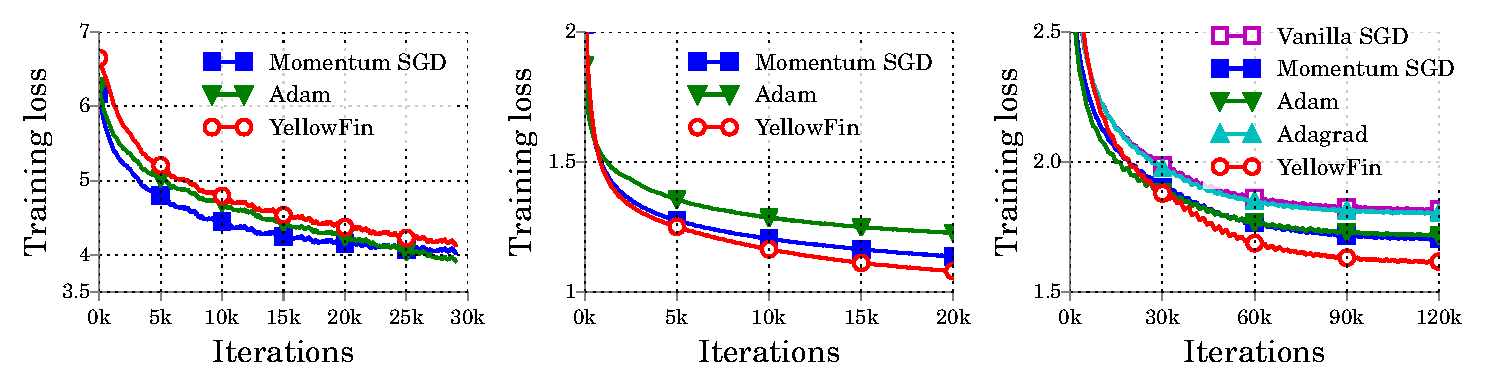
\includegraphics[width=0.925\linewidth]{experiment_results/lstm_loss_all.pdf} \\[-0.5em]
		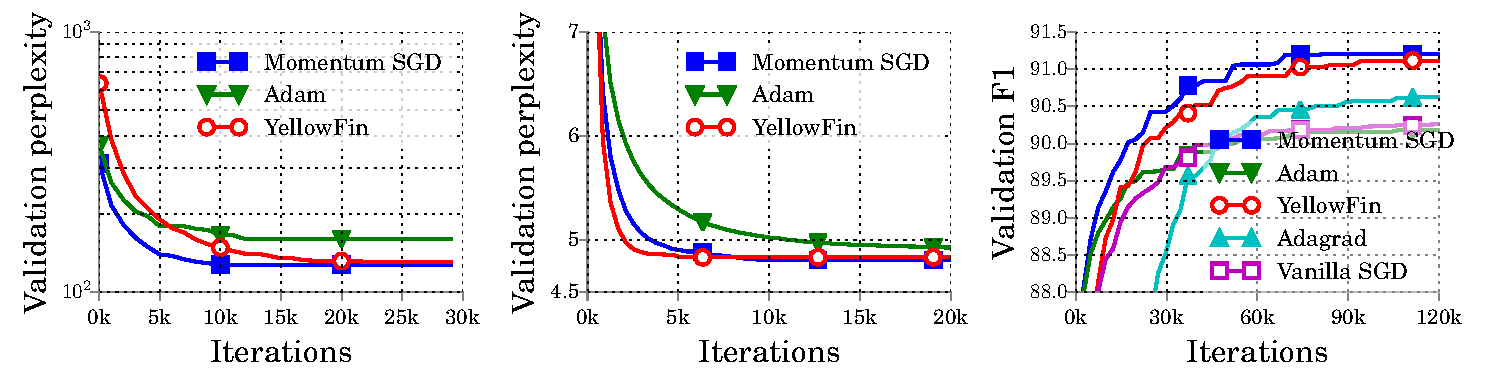
\includegraphics[width=0.925\linewidth]{experiment_results/lstm_test_all.pdf} \\[-0.5em]
	\end{tabular}
%	\vspace{-0.5em}
	\caption{
	Training loss and validation metrics on (left to right) word-level language modeling with PTB, char-level language modeling with TS and constituency parsing on WSJ. The valid. metrics are monotonic as we report the best values up to each number of iterations.}
%	\caption{
%	Training loss and validation metrics on word-level language modeling with PTB (left), char-level language modeling with TS (middle) and constituency parsing on WSJ (right). Note the validation metrics are monotonic as we report the best values up to each specific number of iterations.}
%	\vspace{-0.75em}
	\label{fig:loss_result_ptb}
%	\vspace{-0.25em}
\end{figure*}


%\begin{wrapfigure}[8]{r}{0.42\textwidth}
%\begin{minipage}{1.0\linewidth}
%\vspace{-0.3in}
%%\begin{table}[H]
%%\centering
%%\caption{
%%	Speedup of \tuner and tuned momentum SGD over tuned Adam.
%%	% The speedup is with respect to the number of iterations.
%%	%We compare our Algorithm~\ref{alg:basic-algo}) to the best configuration in tuning grid for Adam and momentum SGD. For tuned Adam and tuned momentum SGD, we take the lowest value of the smoothed training loss curve	 and report the speedup of our  to achieve the same loss. The speedup is demonstrated with respect to the number of iteraions. We run Resnet for 40k iterations, bottleneck resnet for 70k iterations and PTB LSTM for 30k Iterations.
%%	}
%%	\begin{tabular}[t]{c@{\hskip 0.6em}|c@{\hskip 0.6em}c@{\hskip 0.6em}c}
%%		\toprule
%%		 & Adam & mom.SGD & YF \\
%%		\midrule
%%		\midrule
%%		CIFAR10 & 1x & 1.71x & 1.93x  \\
%%		CIFAR100 & 1x & 1.83x & 1.35x \\
%%		PTB & 1x & 0.88x & 0.77x \\
%%		TS & 1x & 5.66x & 6.83x \\
%%		WSJ & 1x & 1.33x & 2.33x \\
%%		\bottomrule
%%	\end{tabular}
%%	\label{tab:iters_to_loss}
%%\end{table}
%% grid search version on Adam
%\begin{table}[H]
%\centering
%\caption{
%	Speedup of \tuner and tuned momentum SGD over tuned Adam.
%	% The speedup is with respect to the number of iterations.
%	%We compare our Algorithm~\ref{alg:basic-algo}) to the best configuration in tuning grid for Adam and momentum SGD. For tuned Adam and tuned momentum SGD, we take the lowest value of the smoothed training loss curve	 and report the speedup of our  to achieve the same loss. The speedup is demonstrated with respect to the number of iteraions. We run Resnet for 40k iterations, bottleneck resnet for 70k iterations and PTB LSTM for 30k Iterations.
%	}
%	\begin{tabular}[t]{c@{\hskip 0.6em}|c@{\hskip 0.6em}c@{\hskip 0.6em}c}
%		\toprule
%		 & Adam & mom.SGD & YF \\
%		\midrule
%		\midrule
%		CIFAR10 & 1x & 1.71x & 1.93x \\
%		CIFAR100 & 1x & 1.87x & 1.38x \\
%		PTB & 1x & 0.88x & 0.77x \\
%		TS & 1x & 2.49x & 3.28x \\
%		WSJ & 1x & 1.33x & 2.33x \\
%		\bottomrule
%	\end{tabular}
%	\label{tab:iters_to_loss}
%\end{table}
%\end{minipage}
%\end{wrapfigure}
We tune Adam and  momentum SGD on learning rate grids with prescribed momentum $0.9$ for SGD. We fix the parameters of Algorithm~\ref{alg:basic-algo} in all experiments, i.e.\ \tuner runs {\em without any hand tuning}.
We provide full specifications, including the learning rate (grid) and the number of iterations we train on each model in Appendix~\ref{sec:exp_spec}.
For visualization purposes, we smooth training losses with a uniform window of width $1000$. 
%\emph{We average the smoothed losses from 3 different random seeds}.
For Adam and momentum SGD on each model, we pick the configuration achieving the lowest averaged smoothed loss.
%in corresponding grids.
To compare two algorithms, we record the lowest smoothed loss achieved by both. Then the speedup is reported as the ratio of iterations to achieve this loss.
We use this setup to validate our claims.
%We tune momentum SGD and Adam on learning rate grids with prescribed momentum $0.9$ for SGD. We fix the parameters of Algorithm~\ref{alg:basic-algo} in all experiments, i.e.\ \tuner runs without any hand tuning. We provide full specifications, including the learning rate (grid) and the number of iterations we train on each model in Appendix~\ref{sec:exp_spec}.
%For visualization purposes, we smooth training losses with a uniform window of width $1000$. 
%%\emph{We average the smoothed losses from 3 different random seeds}.
%For Adam and momentum SGD on each model, we pick the configuration achieving the lowest averaged smoothed loss.
%%in corresponding grids.
%To compare two algorithms, we record the lowest smoothed loss achieved by both. Then the speedup is reported as the ratio of iterations to achieve this loss.
%We use this setup to validate our claims.
%

%%\begin{figure}[t]
%%\centering
%%	\begin{tabular}{c c}
%%		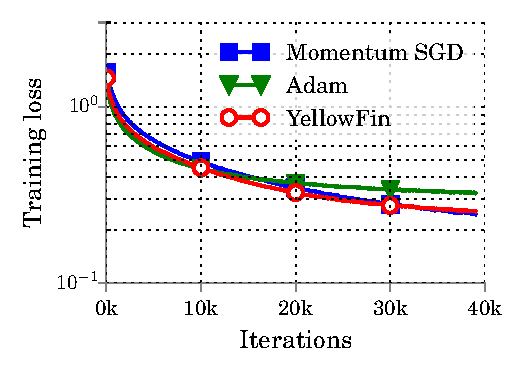
\includegraphics[width=0.45\linewidth]{experiment_results/resnet/resnet_loss.pdf} &
%%		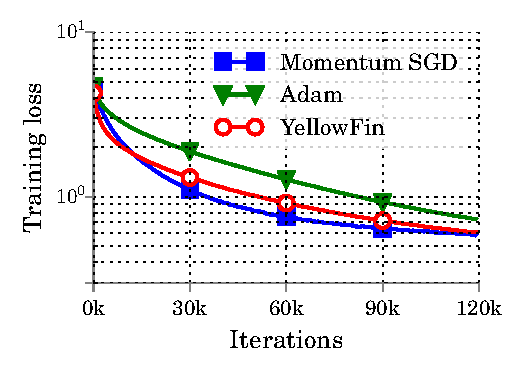
\includegraphics[width=0.45\linewidth]{experiment_results/resnet/resnet_bottleneck_loss.pdf}
%%	\end{tabular}
%%	\caption{
%%	Training loss for ResNet on CIFAR10 (left) and CIFAR100 (right, still running). }
%%	\label{fig:loss_result_cifar}
%%\end{figure}
%
%\begin{wrapfigure}[11]{r}{0.525\textwidth}
%\begin{minipage}{1.0\linewidth}
%\vspace{-0.3in}
%\begin{table}[H]
%\centering
%\caption{
%	The speedup of \tuner and tuned mom. SGD comparing to tuned Adam.
%	% The speedup is with respect to the number of iterations.
%	%We compare our Algorithm~\ref{alg:basic-algo}) to the best configuration in tuning grid for Adam and momentum SGD. For tuned Adam and tuned momentum SGD, we take the lowest value of the smoothed training loss curve	 and report the speedup of our  to achieve the same loss. The speedup is demonstrated with respect to the number of iteraions. We run Resnet for 40k iterations, bottleneck resnet for 70k iterations and PTB LSTM for 30k Iterations.
%	}
%	\begin{tabular}[t]{c@{\hskip 0.6em}|c@{\hskip 0.6em}c@{\hskip 0.6em}c}
%		\toprule
%		 & Adam & mom. SGD & \tuner \\
%		\midrule
%		\midrule
%		CIFAR10 & 1x & 1.71x & 1.93x \\
%		CIFAR100 & 1x & 1.87x & 1.38x \\
%		PTB & 1x & 0.88x & 0.77x \\
%		TS & 1x & 2.49x & 3.28x \\
%		WSJ & 1x & 1.33x & 2.33x \\
%		\bottomrule
%	\end{tabular}
%	\label{tab:iters_to_loss}
%\end{table}
%\end{minipage}
%\end{wrapfigure}
%\begin{wrapfigure}[11]{r}{0.39\textwidth}
%\begin{minipage}{1.0\linewidth}
%\vspace{-0.15in}
%%\begin{table}[H]
%%\centering
%%\caption{
%%	Speedup of \tuner and tuned momentum SGD over tuned Adam.
%%	% The speedup is with respect to the number of iterations.
%%	%We compare our Algorithm~\ref{alg:basic-algo}) to the best configuration in tuning grid for Adam and momentum SGD. For tuned Adam and tuned momentum SGD, we take the lowest value of the smoothed training loss curve	 and report the speedup of our  to achieve the same loss. The speedup is demonstrated with respect to the number of iteraions. We run Resnet for 40k iterations, bottleneck resnet for 70k iterations and PTB LSTM for 30k Iterations.
%%	}
%%	\begin{tabular}[t]{c@{\hskip 0.6em}|c@{\hskip 0.6em}c@{\hskip 0.6em}c}
%%		\toprule
%%		 & Adam & mom.SGD & YF \\
%%		\midrule
%%		\midrule
%%		CIFAR10 & 1x & 1.71x & 1.93x  \\
%%		CIFAR100 & 1x & 1.83x & 1.35x \\
%%		PTB & 1x & 0.88x & 0.77x \\
%%		TS & 1x & 5.66x & 6.83x \\
%%		WSJ & 1x & 1.33x & 2.33x \\
%%		\bottomrule
%%	\end{tabular}
%%	\label{tab:iters_to_loss}
%%\end{table}
%% grid search version on Adam
%\begin{table}[H]
%\centering
%\caption{
%	Speedup of \tuner and tuned mom. SGD over tuned Adam.
%	% The speedup is with respect to the number of iterations.
%	%We compare our Algorithm~\ref{alg:basic-algo}) to the best configuration in tuning grid for Adam and momentum SGD. For tuned Adam and tuned momentum SGD, we take the lowest value of the smoothed training loss curve	 and report the speedup of our  to achieve the same loss. The speedup is demonstrated with respect to the number of iteraions. We run Resnet for 40k iterations, bottleneck resnet for 70k iterations and PTB LSTM for 30k Iterations.
%	}
%	\begin{tabular}[t]{@{\hskip 0.3em}c@{\hskip 0.3em}|c@{\hskip 0.3em}c@{\hskip 0.3em}c@{\hskip 0.3em}}
%		\toprule
%		 & Adam & mom.SGD & YF \\
%		\midrule
%		\midrule
%		CIFAR10 & $1\times$ & $1.71\times$ & $1.93\times$ \\
%		CIFAR100 & $1\times$ & $1.87\times$ & $1.38\times$ \\
%		PTB & $1\times$ & $0.88\times$ & $0.77\times$ \\
%		TS & $1\times$ & $2.49\times$ & $3.28\times$ \\
%		WSJ & $1\times$ & $1.33\times$ & $2.33\times$ \\
%		\bottomrule
%	\end{tabular}
%	\label{tab:iters_to_loss}
%\end{table}
%\end{minipage}
%\end{wrapfigure}

%\begin{wrapfigure}[10]{r}{0.375\textwidth}
%\begin{minipage}{1.0\linewidth}
%\vspace{-0.35in}
%\begin{table}[H]
%\centering
%\caption{
%	Speedup of \tuner and tuned momentum SGD over tuned Adam.
%	% The speedup is with respect to the number of iterations.
%	%We compare our Algorithm~\ref{alg:basic-algo}) to the best configuration in tuning grid for Adam and momentum SGD. For tuned Adam and tuned momentum SGD, we take the lowest value of the smoothed training loss curve	 and report the speedup of our  to achieve the same loss. The speedup is demonstrated with respect to the number of iteraions. We run Resnet for 40k iterations, bottleneck resnet for 70k iterations and PTB LSTM for 30k Iterations.
%	}
%	\begin{tabular}[t]{c@{\hskip 0.6em}|c@{\hskip 0.6em}c@{\hskip 0.6em}c}
%		\toprule
%		 & Adam & mom.SGD & YF \\
%		\midrule
%		\midrule
%		CIFAR10 & 1x & 1.71x & 1.93x  \\
%		CIFAR100 & 1x & 1.83x & 1.35x \\
%		PTB & 1x & 0.88x & 0.77x \\
%		TS & 1x & 5.66x & 6.83x \\
%		WSJ & 1x & 1.33x & 2.33x \\
%		\bottomrule
%	\end{tabular}
%	\label{tab:iters_to_loss}
%\end{table}
% grid search version on Adam
%%%%%%%%%%%%%%% old version table %%%%%%%%%%%%%%%%%%%
%\begin{table}[H]
%\centering
%\caption{
%	Speedup of \tuner and tuned mom. SGD over tuned Adam.
%	% The speedup is with respect to the number of iterations.
%	%We compare our Algorithm~\ref{alg:basic-algo}) to the best configuration in tuning grid for Adam and momentum SGD. For tuned Adam and tuned momentum SGD, we take the lowest value of the smoothed training loss curve	 and report the speedup of our  to achieve the same loss. The speedup is demonstrated with respect to the number of iteraions. We run Resnet for 40k iterations, bottleneck resnet for 70k iterations and PTB LSTM for 30k Iterations.
%	}
%%	\vspace{-0.075in}
%%	\begin{tabular}[t]{@{\hskip 0.15em}c@{\hskip 0.15em}|c@{\hskip 0.3em}c@{\hskip 0.3em}c@{\hskip 0.15em}}
%	\begin{tabular}{c | c c c}
%		 & Adam & mom.SGD & YF \\
%		\midrule
%		\midrule
%%		CIFAR10 & $1\times$ & $1.71\times$ & $1.93\times$ \\
%%		CIFAR100 & $1\times$ & $1.87\times$ & $1.38\times$ \\
%%		PTB & $1\times$ & $0.88\times$ & $0.77\times$ \\
%%		TS & $1\times$ & $2.49\times$ & $3.28\times$ \\
%%		WSJ & $1\times$ & $1.33\times$ & $2.33\times$ \\
%		CIFAR10 & 1x & 1.71x & 1.93x \\
%		CIFAR100 & 1x & 1.87x & 1.38x \\
%		PTB & 1x & 0.88x & 0.77x \\
%		TS & 1x & 2.49x & 3.28x \\
%		WSJ & 1x & 1.33x & 2.33x \\
%		\bottomrule
%	\end{tabular}
%	\label{tab:iters_to_loss}
%\end{table}
%%%%%%%%%%%%%%%%%%%%%%%%%%%%%%%%%%%%%%%%%%%%%%%%%%%%%
%%%%%%%%%%%%%%% new version table %%%%%%%%%%%%%%%%%%%
\vspace{-0.25em}
\begin{table}[h]
\centering
\small
%	\begin{tabular}[t]{@{\hskip 0.3em}c@{\hskip 0.5em}|c@{\hskip 0.45em}c@{\hskip 0.45em}c@{\hskip 0.75em}c@{\hskip 0.75em}c@{\hskip 0.15em}}
	\begin{tabular}[t]{@{\hskip 0.5em}c@{\hskip 0.5em}|c@{\hskip 1em}c@{\hskip 1em}c@{\hskip 1em}c@{\hskip 1em}c@{\hskip 0.5em}}
%	\begin{tabular}{c | c c c c c}
		\toprule
		 & CIFAR10 & CIFAR100 & PTB & TS & WSJ \\
		\midrule
		\midrule
		Adam & 1x & 1x & 1x & 1x & 1x \\
		mom. SGD & 1.71x & 1.87x & 0.88x & 2.49x & 1.33x \\
		YF & 1.93x & 1.38x & 0.77x & 3.28x & 2.33x \\
%		CIFAR10 & 1x & 1.71x & 1.93x \\
%		CIFAR100 & 1x & 1.87x & 1.38x \\
%		PTB & 1x & 0.88x & 0.77x \\
%		TS & 1x & 2.49x & 3.28x \\
%		WSJ & 1x & 1.33x & 2.33x \\
		\bottomrule
	\end{tabular}
	\caption{
	The speedup of \tuner and tuned momentum SGD over tuned Adam on ResNet and LSTM models.
	% The speedup is with respect to the number of iterations.
	%We compare our Algorithm~\ref{alg:basic-algo}) to the best configuration in tuning grid for Adam and momentum SGD. For tuned Adam and tuned momentum SGD, we take the lowest value of the smoothed training loss curve	 and report the speedup of our  to achieve the same loss. The speedup is demonstrated with respect to the number of iteraions. We run Resnet for 40k iterations, bottleneck resnet for 70k iterations and PTB LSTM for 30k Iterations.
	}
	\label{tab:iters_to_loss}
%	\vspace{-0.85em}
\end{table}
\vspace{-0.5em}

%%%%%%%%%%%%%%%%%%%%%%%%%%%%%%%%%%%%%%%%%%%%%%%%%%%%%
%\end{minipage}
%\end{wrapfigure}
\paragraph{Momentum SGD is competitive with adaptive methods}
In Table~\ref{tab:iters_to_loss}, we compare tuned momentum SGD and tuned Adam on ResNets with training losses shown in Figure~\ref{fig:loss_result_cifar} in Appendix~\ref{sec:add_exp}. We can observe that momentum SGD
achieves $1.71$x and $1.87$x speedup to tuned Adam on CIFAR10 and CIFAR100 respectively. In Figure~\ref{fig:loss_result_ptb} and Table~\ref{tab:iters_to_loss}, 
with the exception of PTB LSTM, momentum SGD also produces better training loss, as well as better validation perplexity in language modeling and validation F1 in parsing.
For the parsing task, we also compare with tuned Vanilla SGD and AdaGrad, which are used in the NLP community.
Figure~\ref{fig:loss_result_ptb} (right) shows that \emph{fixed momentum 0.9 can already speedup Vanilla SGD by $2.73$x, achieving observably better validation F1}. %,
%a performance matched by \tuner. 
 We refer to Appendix~\ref{sec:importance_momentum} for further discussion on the importance of momentum adaptivity in \tuner.
%These observations show that momentum is critical to acceleration, and momentum SGD can be better than the state-of-the-art adaptive method in a variety of models.% 

%\begin{figure*}[t]
%%\vspace{-2.25em}
%\centering
%	\begin{tabular}{c}
%		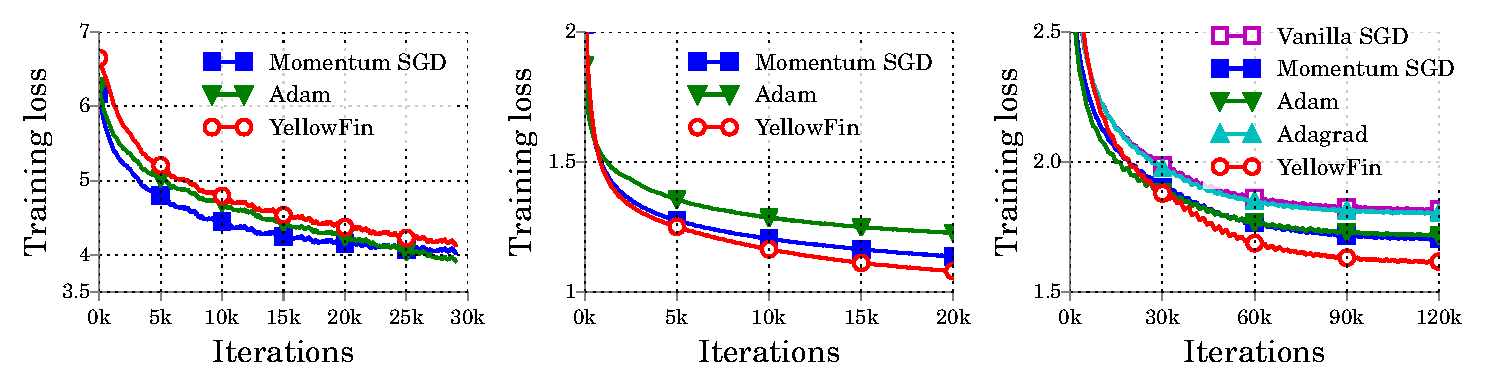
\includegraphics[width=0.925\linewidth]{experiment_results/lstm_loss_all.pdf} \\[-0.75em]
%		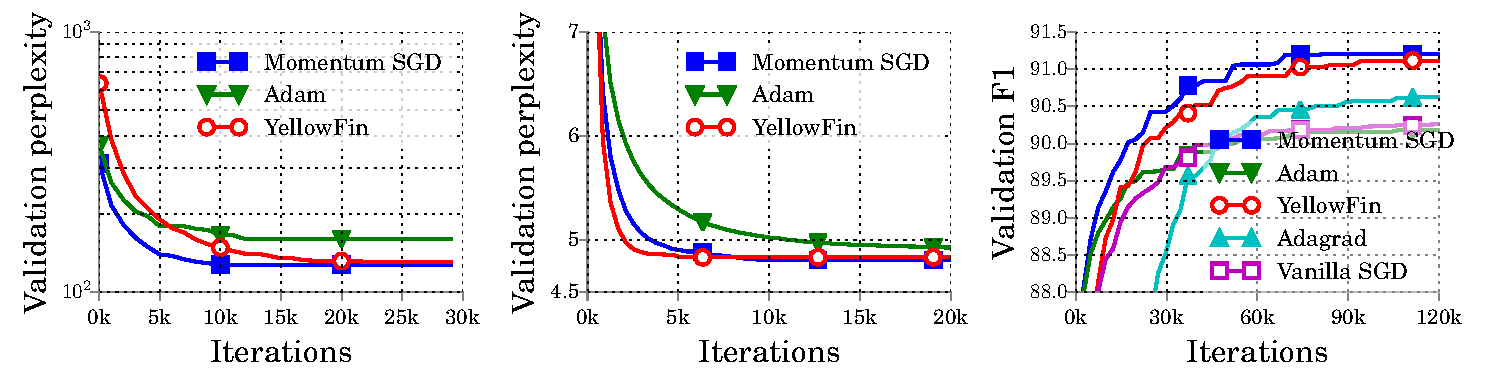
\includegraphics[width=0.925\linewidth]{experiment_results/lstm_test_all.pdf} \\[-0.5em]
%	\end{tabular}
%	\caption{
%	Training loss and test metrics on word-level language modeling with PTB (left), character-level language modeling with TS (middle) and constituency parsing on WSJ (right). Note the validation metrics are monotonic as we report the best values up to each specific number of iterations.}
%	\vspace{-0.75em}
%	\label{fig:loss_result_ptb}
%\end{figure*}


%\begin{wrapfigure}[10]{r}{0.375\textwidth}
%\begin{minipage}{1.0\linewidth}
%\vspace{-0.35in}
%%\begin{table}[H]
%%\centering
%%\caption{
%%	Speedup of \tuner and tuned momentum SGD over tuned Adam.
%%	% The speedup is with respect to the number of iterations.
%%	%We compare our Algorithm~\ref{alg:basic-algo}) to the best configuration in tuning grid for Adam and momentum SGD. For tuned Adam and tuned momentum SGD, we take the lowest value of the smoothed training loss curve	 and report the speedup of our  to achieve the same loss. The speedup is demonstrated with respect to the number of iteraions. We run Resnet for 40k iterations, bottleneck resnet for 70k iterations and PTB LSTM for 30k Iterations.
%%	}
%%	\begin{tabular}[t]{c@{\hskip 0.6em}|c@{\hskip 0.6em}c@{\hskip 0.6em}c}
%%		\toprule
%%		 & Adam & mom.SGD & YF \\
%%		\midrule
%%		\midrule
%%		CIFAR10 & 1x & 1.71x & 1.93x  \\
%%		CIFAR100 & 1x & 1.83x & 1.35x \\
%%		PTB & 1x & 0.88x & 0.77x \\
%%		TS & 1x & 5.66x & 6.83x \\
%%		WSJ & 1x & 1.33x & 2.33x \\
%%		\bottomrule
%%	\end{tabular}
%%	\label{tab:iters_to_loss}
%%\end{table}
%% grid search version on Adam
%\begin{table}[H]
%\centering
%\caption{
%	Speedup of \tuner and tuned mom. SGD over tuned Adam.
%	% The speedup is with respect to the number of iterations.
%	%We compare our Algorithm~\ref{alg:basic-algo}) to the best configuration in tuning grid for Adam and momentum SGD. For tuned Adam and tuned momentum SGD, we take the lowest value of the smoothed training loss curve	 and report the speedup of our  to achieve the same loss. The speedup is demonstrated with respect to the number of iteraions. We run Resnet for 40k iterations, bottleneck resnet for 70k iterations and PTB LSTM for 30k Iterations.
%	}
%	\vspace{-0.075in}
%	\begin{tabular}[t]{@{\hskip 0.15em}c@{\hskip 0.15em}|c@{\hskip 0.3em}c@{\hskip 0.3em}c@{\hskip 0.15em}}
%		\toprule
%		 & Adam & mom.SGD & YF \\
%		\midrule
%		\midrule
%%		CIFAR10 & $1\times$ & $1.71\times$ & $1.93\times$ \\
%%		CIFAR100 & $1\times$ & $1.87\times$ & $1.38\times$ \\
%%		PTB & $1\times$ & $0.88\times$ & $0.77\times$ \\
%%		TS & $1\times$ & $2.49\times$ & $3.28\times$ \\
%%		WSJ & $1\times$ & $1.33\times$ & $2.33\times$ \\
%		CIFAR10 & 1x & 1.71x & 1.93x \\
%		CIFAR100 & 1x & 1.87x & 1.38x \\
%		PTB & 1x & 0.88x & 0.77x \\
%		TS & 1x & 2.49x & 3.28x \\
%		WSJ & 1x & 1.33x & 2.33x \\
%		\bottomrule
%	\end{tabular}
%	\label{tab:iters_to_loss}
%\end{table}
%\end{minipage}
%\end{wrapfigure}
\paragraph{\tuner can match hand-tuned momentum SGD and can outperform hand-tuned Adam}% on ResNets and LSTMs}
In our experiments, 
\tuner, without any hand-tuning, yields training loss matching hand-tuned momentum SGD for all the ResNet and LSTM models in Figure~\ref{fig:loss_result_ptb} and~\ref{fig:loss_result_cifar}.  
When comparing to tuned Adam in Table~\ref{tab:iters_to_loss}, except being slightly slower on PTB LSTM, \tuner achieves $1.38$x to $3.28$x speedups in training losses on the other four models. \emph{More importantly, \tuner consistently shows better validation metrics than tuned Adam in Figure~\ref{fig:loss_result_ptb}}. It demonstrates that \tuner can match tuned momentum SGD and outperform tuned state-of-the-art adaptive optimizers. % in training deep neural networks.% in a large class of models.
In Appendix~\ref{sec:boost_exp}, we show \tuner further speeding up with finer-grain manual learning rate tuning.
%As careful optimizer tuning can further improve model performance in fixed training time, we refer to Appendix~\ref{sec:boost_exp} on auxiliary manual learning rate tuning for \tuner.

%%In our experiments, 
%%\tuner, without any hand-tuning, yields speedups from to 1.32x to 3.28x on ResNets and LSTMs in comparison to tuned momentum SGD.  
%When comparing to tuned Adam in Table~\ref{tab:iters_to_loss}, \tuner achieves speedups from 1.32x to 3.28x in training losses. \emph{More importantly, \tuner consistently shows better test metrics than tuned momentum SGD and Adam}. It demonstrates that \tuner can outperform hand-tuned state-of-the-art adaptive and non-adaptive optimizers.% in a large class of models.
\begin{figure*}
\centering	
\begin{tabular}{c c c}
	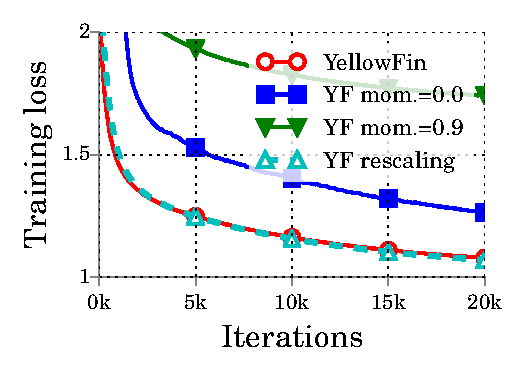
\includegraphics[width=0.31\linewidth]{experiment_results/tf_charrnn_train_loss_fix_mom_and_lr_rescaling_cmp.pdf} &
	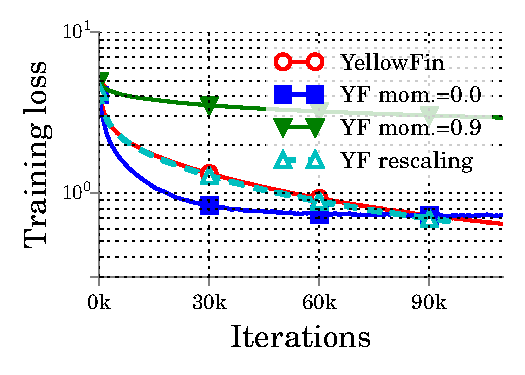
\includegraphics[width=0.31\linewidth]{experiment_results/resnet/resnet_bottleneck_loss_fix_mom_and_lr_rescaling_cmp} &
	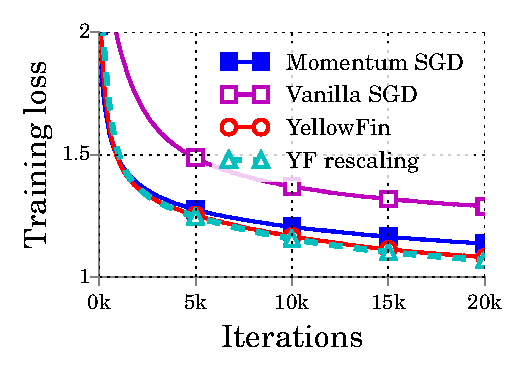
\includegraphics[width=0.31\linewidth]{experiment_results/tf_charrnn_train_loss_mom_vanilla_yf.pdf}
\end{tabular}
\caption{The importance of adaptive momentum: Training loss comparison between \tuner with adaptive momentum and \tuner with fixed momentum value; this comparison is conducted on TS LSTM (left) and CIFAR100 ResNet (right). Learning rate scaling based on \tuner tuned momentum can match the performance of full \tuner (right) on the TS LSTM. However without the \tuner tuned momentum, hand-tuned Vanilla SGD demonstrates observably larger training loss than momentum based methods, including full \tuner, \tuner learning rate rescaling and hand-tuned momentum SGD (with the same learning rate search grid as with Vanilla SGD.)}
\label{fig:cmp_fix_mom}
\end{figure*}

\paragraph{The importance of adaptive momentum in \tuner}
In Definition~\ref{def:GCN}, we noticed that the optimally tuned $\mu^*$ is highly objective-dependent. Empirically, We indeed observe a wide range of tuned momentum $\mu$ from YF; it ranges from smaller than 0.03 in the PTM LSTM to 0.89 for ResNext. To further validate the importance of momentum adaptivity in \tuner, we perform an ablation study to demonstrate the importance of objective-dependent momentum adaptivity in \tuner with CIFAR100 ResNet and TS LSTM. In the experiments, \tuner tunes the learning rate. Instead of also using the momentum tuned by YF, we continuously feed objective-agnostic prescribed momentum value $0.0$ and $0.9$ to the underlying momentum SGD optimizer which YF is tuning. In Figure~\ref{fig:cmp_fix_mom}, when comparing to \tuner with prescribed momentum 0.0 or 0.9, \tuner with adaptively tuned momentum achieves observably faster convergence on both TS LSTM and CIFAR100 ResNet. From a more practical perspective, in Figure~\ref{fig:loss_result_ptb} (bottom right) and Figure~\ref{fig:cmp_fix_mom} (right), we also observe that hand-tuned optimizer without momentum, i.e. Vanilla SGD, typically can not match the performance of momentum based methods, including \tuner and momentum SGD hand-tuned using the same learning rate grid as with Vanilla SGD. However in \tuner, we can rescale the learning rate based on the \tuner tuned momentum $\mu_t$, and use 0 momentum in the model updates to match the performance of momentum based methods. Specifically, we rescale the \tuner tuned learning rate $\alpha_t$ with $1/(1 - \mu_t)$ \footnote{Let $v_t = x_t - x_{t - 1}$ be the model update, this rescaling is motivated with the fact that $v_{t+1} = \mu_t v_{t} - \alpha_t \nabla f(x_t)$. Assuming the $v_t$ evolves smoothly, we have $v_t \approx \alpha_t/(1-\mu_t) \nabla f(x_t)$.}. Model updates with this rescaled learning rate and 0 momentum can demonstrate training loss closely matching those of \tuner and hand-tuned momentum SGD for WSJ LSTM in Figure~\ref{fig:loss_result_ptb} (bottom right) and TS LSTM in Figure~\ref{fig:cmp_fix_mom} (right).



%\begin{wrapfigure}[9]{r}{0.34\linewidth}
%\vspace{-0.6in}
%\begin{minipage}{1.0\linewidth}
%	\begin{figure}[H]
%		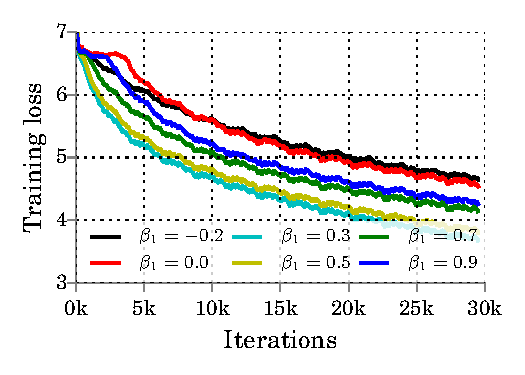
\includegraphics[width=0.975\linewidth]{experiment_results/ptb/adam_stale_15_tuning.pdf}
%			\vspace{-1.5em}
%		\caption{Hand-tuning Adam's momentum under asynchrony.}
%		\label{fig:adam_async_mom}
%	\end{figure}
%%	\vspace{-1.5em}
%%	\begin{figure}[H]
%%		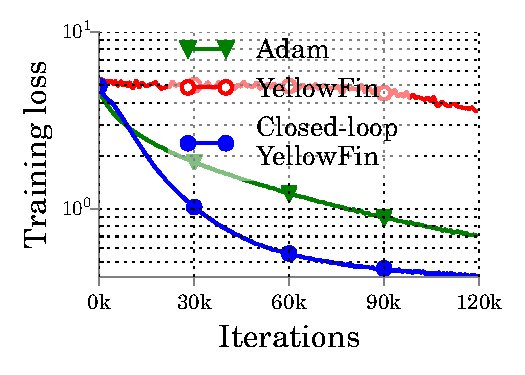
\includegraphics[width=0.975\linewidth]{experiment_results/resnet/resnet_bottleneck_cmp_tuner_adam.pdf}
%%%		\caption{Adam, \tuner and \asynctuner on CIFAR100 with 16 async. workers. Sync. baseline uses \tuner.}
%%	\vspace{-1.5em}
%%		\caption{Asynchronous performance on CIFAR100 ResNet.}
%%		\label{fig:full_async_cmp}
%%	\end{figure}
%\end{minipage}	
%\end{wrapfigure}

%\begin{wrapfigure}[9]{R}{0.5\linewidth}
%\vspace{-0.575in}
%%\vspace{-0.75in}
%\begin{minipage}{\linewidth}
%%	\begin{figure}[H]
%%		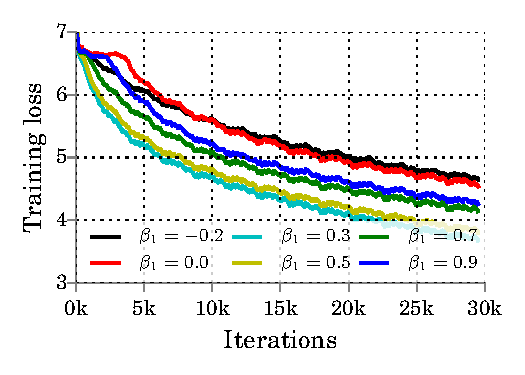
\includegraphics[width=\linewidth]{experiment_results/ptb/adam_stale_15_tuning.pdf}
%%			\vspace{-1.5em}
%%		\caption{Hand-tuning Adam's momentum under asynchrony.}
%%		\label{fig:adam_async_mom}
%%	\end{figure}
%%	\vspace{-1.5em}
%	\begin{figure}[H]
%		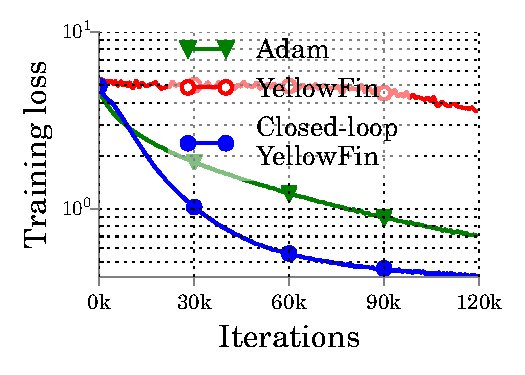
\includegraphics[width=1.05\linewidth]{experiment_results/resnet/resnet_bottleneck_cmp_tuner_adam.pdf}
%%		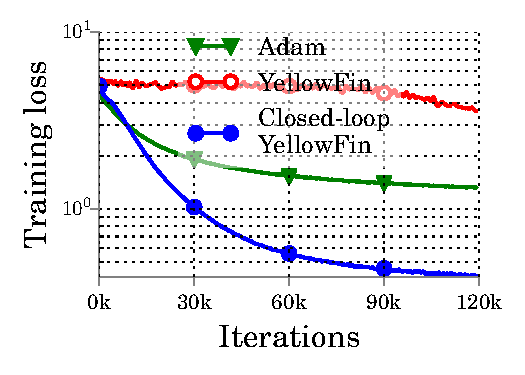
\includegraphics[width=0.975\linewidth]{experiment_results/resnet/resnet_bottleneck_cmp_tuner_adam_default_adam.pdf}
%%		\caption{Adam, \tuner and \asynctuner on CIFAR100 with 16 async. workers. Sync. baseline uses \tuner.}
%	\vspace{-1.75em}
%		\caption{Asynchronous performance on CIFAR100 ResNet.}
%		\label{fig:full_async_cmp}
%	\end{figure}
%\end{minipage}	
%\end{wrapfigure}
%%\vspace*{5.0em}
\subsection{Asynchronous experiments}
\label{sec:async_exp}
%\vspace{-1em}
In this section, we evaluate \asynctuner with focus on the number of iterations to reach a certain solution. 
To that end, we run $16$ asynchronous workers on a single machine and force them to update the model in a round-robin fashion,
i.e. the gradient is delayed for $15$ iterations.
%We demonstrate
%%(1) Adam suffers a convergence speed penalty due to not tuning momentum in asynchronous settings;
%(1) \asynctuner (cf.\ Section~\ref{sec:async_tuner}) improves the convergence of \tuner dramatically, which leads to
%(3) \asynctuner having much faster convergence than Adam. 
%     
%\paragraph{State-of-the-art adaptive methods suffer from lack of momentum tuning} We conduct experiments on PTB LSTM with 16 asynchronous workers using Adam.
%Fixing the learning rate to the value achieving the lowest smoothed loss in Section~\ref{subsec:sync_exp}, we sweep the smoothing parameter $\beta_1$~\citep{kingma2014adam} of the first order moment estimate in grid $\{-0.2, 0.0, 0.3, 0.5, 0.7, 0.9\}$. $\beta_1$ serves the same role as momentum in SGD and we call it the momentum in Adam. Figure~\ref{fig:adam_async_mom} shows tuning momentum for Adam under asynchrony gives measurably better training loss. 
%This result emphasizes the importance of momentum tuning in asynchronous settings and suggests that state-of-the-art adaptive methods pay a penalty for using prescribed momentum.
%
%\begin{wrapfigure}[10]{r}{0.34\linewidth}
%\vspace{-0.35in}
%\begin{minipage}{1.0\linewidth}
%%	\begin{figure}[H]
%%		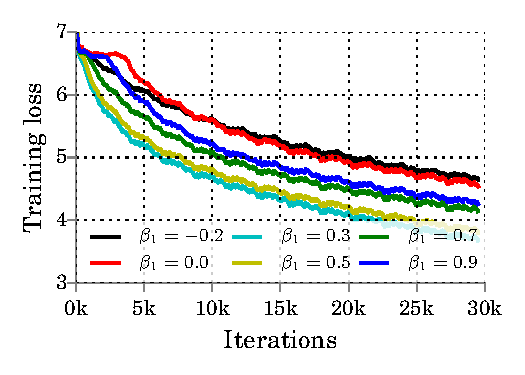
\includegraphics[width=\linewidth]{experiment_results/ptb/adam_stale_15_tuning.pdf}
%%			\vspace{-1.5em}
%%		\caption{Hand-tuning Adam's momentum under asynchrony.}
%%		\label{fig:adam_async_mom}
%%	\end{figure}
%%	\vspace{-1.5em}
%	\begin{figure}[H]
%		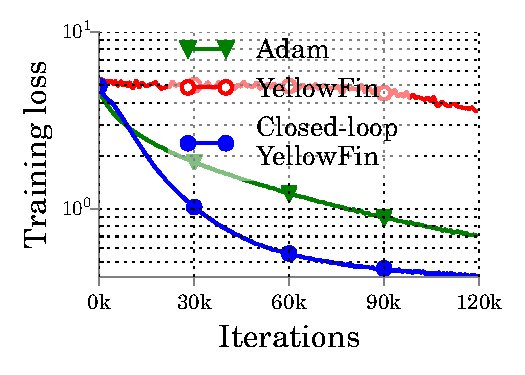
\includegraphics[width=0.975\linewidth]{experiment_results/resnet/resnet_bottleneck_cmp_tuner_adam.pdf}
%%		\caption{Adam, \tuner and \asynctuner on CIFAR100 with 16 async. workers. Sync. baseline uses \tuner.}
%	\vspace{-1.5em}
%		\caption{Asynchronous performance on CIFAR100 ResNet.}
%		\label{fig:full_async_cmp}
%	\end{figure}
%\end{minipage}	
%\end{wrapfigure}
%\paragraph{Closing the loop improves convergence under staleness}
%We compare the performance of \tuner in Algorithm~\ref{alg:basic-algo} and \asynctuner in Algorithm~\ref{alg:async-algo} on the 164-layer bottleneck ResNet. We conduct experiments using 16 asynchronous workers.
%In Figure~\ref{fig:adam_under_staleness} (right), 
%Figure~\ref{fig:full_async_cmp} 
Figure~\ref{fig:spotlight} (right) 
presents training losses on the CIFAR100 ResNet, using \tuner in Algorithm~\ref{alg:basic-algo}, \asynctuner in Algorithm~\ref{alg:async-algo} and Adam with the learning rate achieving the best smoothed loss in Section~\ref{subsec:sync_exp}.
We can observe closed-loop \tuner achieves $20.1$x speedup to \tuner, 
%Consequently, closed-loop \tuner achieves 5.09x speedup over Adam.
and consequently a $2.69$x speedup to Adam.
This demonstrates that (1) \asynctuner accelerates by reducing algorithmic momentum to compensate for asynchrony and (2) can converge in less iterations than Adam in asynchronous-parallel training. 
%We notice that \asynctuner achieves very similar loss as the synchronous baseline near the end.
%It suggests an almost $16$x wall-clock time speedup by parallelizing asynchronously.
%\vspace{-0.5em}
%\paragraph{Closed-loop \tuner outperforms Adam in asynchrony} 
%We run Adam with 16 workers on CIFAR100 ResNet using the learning rate achieving the lowest smoothed loss in Section~\ref{subsec:sync_exp}.
%Shown in Figure~\ref{fig:full_async_cmp}, Adam slows down dramatically due to asynchrony, while closed-loop \tuner, with feedback gain $\gamma=0.01$, demonstrates up to 2.69x speedup  over Adam.
%It shows \asynctuner can significantly outperform the state-of-the-art in asynchronous settings.

%\begin{figure}[t]
%\centering
%	\begin{tabular}{c c}
%		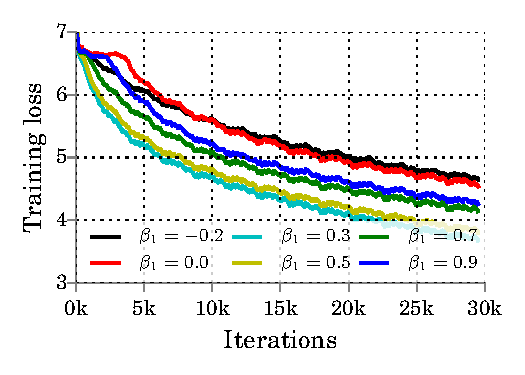
\includegraphics[width=0.45\linewidth]{experiment_results/ptb/adam_stale_15_tuning.pdf} &
%		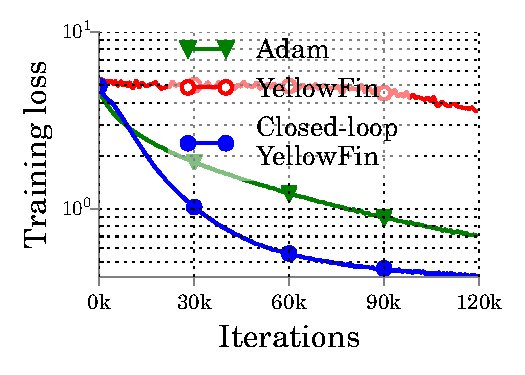
\includegraphics[width=0.45\linewidth]{experiment_results/resnet/resnet_bottleneck_cmp_tuner_adam.pdf}
%	\end{tabular}
%	\caption{
%	Hand-tuning Adam's momentum under asynchrony (left) on PTB LSTM. Asynchronous performance comparison (right) on CIFAR100 ResNet.}
%	\label{fig:adam_under_staleness}
%\end{figure}



%% async experiment backup version
%\begin{wrapfigure}[9]{r}{0.34\linewidth}
%\vspace{-0.6in}
%\begin{minipage}{1.0\linewidth}
%	\begin{figure}[H]
%		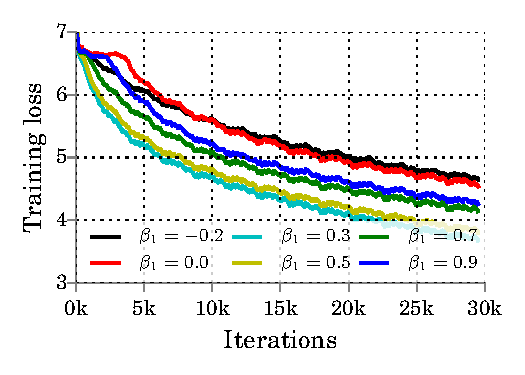
\includegraphics[width=0.975\linewidth]{experiment_results/ptb/adam_stale_15_tuning.pdf}
%			\vspace{-1.5em}
%		\caption{Hand-tuning Adam's momentum under asynchrony.}
%		\label{fig:adam_async_mom}
%	\end{figure}
%%	\vspace{-1.5em}
%%	\begin{figure}[H]
%%		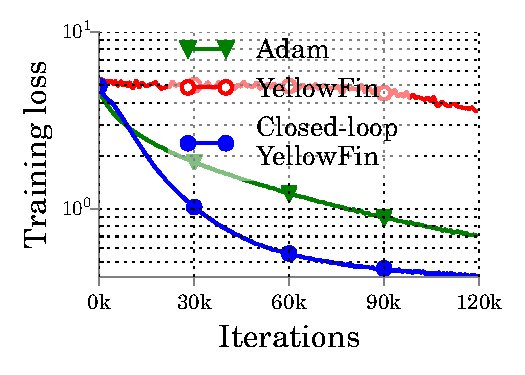
\includegraphics[width=0.975\linewidth]{experiment_results/resnet/resnet_bottleneck_cmp_tuner_adam.pdf}
%%%		\caption{Adam, \tuner and \asynctuner on CIFAR100 with 16 async. workers. Sync. baseline uses \tuner.}
%%	\vspace{-1.5em}
%%		\caption{Asynchronous performance on CIFAR100 ResNet.}
%%		\label{fig:full_async_cmp}
%%	\end{figure}
%\end{minipage}	
%\end{wrapfigure}
%\subsection{Asynchronous experiments}
%In this section, we evaulate \tuner in an asynchronous-parallel setting,
%where we focus on {\em statistical efficiency}: the number of iterations to reach a certain solution. 
%To that end, we run $M$ asynchronous workers on a single machine and force them to update the model in a round-robin fashion,
%i.e. the staled gradient is delayed for $(M-1)$ iterations.
%We demonstrate
%(1) Adam suffers a convergence speed penalty due to not tuning momentum in asynchronous settings;
%(2) \asynctuner (cf.\ Section~\ref{sec:async_tuner}) improves the convergence of \tuner dramatically, which leads to
%(3) \asynctuner having much faster convergence than Adam. 
%     
%
%\paragraph{State-of-the-art adaptive methods suffer from lack of momentum tuning} We conduct experiments on PTB LSTM with 16 asynchronous workers using Adam.
%Fixing the learning rate to the value achieving the lowest smoothed loss in Section~\ref{subsec:sync_exp}, we sweep the smoothing parameter $\beta_1$~\citep{kingma2014adam} of the first order moment estimate in grid $\{-0.2, 0.0, 0.3, 0.5, 0.7, 0.9\}$. $\beta_1$ serves the same role as momentum in SGD and we call it the momentum in Adam. Figure~\ref{fig:adam_async_mom} shows tuning momentum for Adam under asynchrony gives measurably better training loss. 
%This result emphasizes the importance of momentum tuning in asynchronous settings and suggests that state-of-the-art adaptive methods pay a penalty for using prescribed momentum.
%
%\begin{wrapfigure}[10]{r}{0.34\linewidth}
%\vspace{-0.35in}
%\begin{minipage}{1.0\linewidth}
%%	\begin{figure}[H]
%%		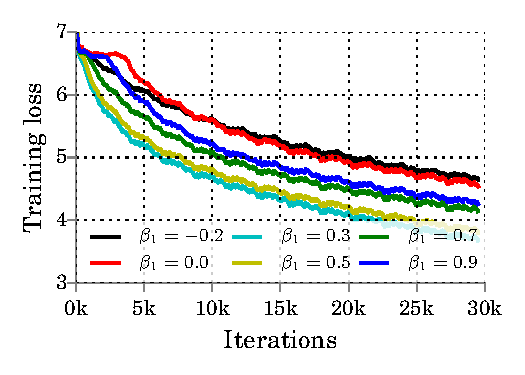
\includegraphics[width=\linewidth]{experiment_results/ptb/adam_stale_15_tuning.pdf}
%%			\vspace{-1.5em}
%%		\caption{Hand-tuning Adam's momentum under asynchrony.}
%%		\label{fig:adam_async_mom}
%%	\end{figure}
%%	\vspace{-1.5em}
%	\begin{figure}[H]
%		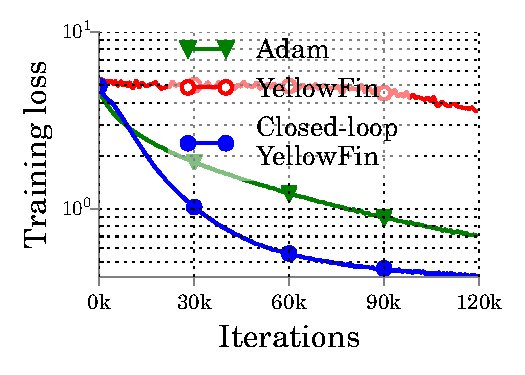
\includegraphics[width=0.975\linewidth]{experiment_results/resnet/resnet_bottleneck_cmp_tuner_adam.pdf}
%%		\caption{Adam, \tuner and \asynctuner on CIFAR100 with 16 async. workers. Sync. baseline uses \tuner.}
%	\vspace{-1.5em}
%		\caption{Asynchronous performance on CIFAR100 ResNet.}
%		\label{fig:full_async_cmp}
%	\end{figure}
%\end{minipage}	
%\end{wrapfigure}
%\paragraph{Closing the loop improves convergence under staleness}
%We compare the performance of \tuner in Algorithm~\ref{alg:basic-algo} and \asynctuner in Algorithm~\ref{alg:async-algo} on the 164-layer bottleneck ResNet. We conduct experiments using 16 asynchronous workers.
%%In Figure~\ref{fig:adam_under_staleness} (right), 
%In Figure~\ref{fig:full_async_cmp}, 
%we observe \tuner without closed-loop momentum control decrease slowly before 90k iterations. Consequently, the closed-loop \tuner achieves more than 20.1x speedup to reach the lowest loss from \tuner after 120k iterations.
%This demonstrates that \asynctuner accelerates by effectively reducing algorithmic momentum to compensate for asynchrony. 
%%We notice that \asynctuner achieves very similar loss as the synchronous baseline near the end.
%%It suggests an almost $16$x wall-clock time speedup by parallelizing asynchronously.
%\vspace{-0.5em}
%\paragraph{Closed-loop \tuner outperforms Adam in asynchrony} We run Adam with 16 workers on CIFAR100 ResNet using the learning rate achieving the lowest smoothed loss in Section~\ref{subsec:sync_exp}.
%Shown in Figure~\ref{fig:full_async_cmp}, Adam slows down dramatically due to asynchrony, while closed-loop \tuner, with feedback gain $\gamma=0.01$, demonstrates up to 2.69x speedup  over Adam.
%%It shows \asynctuner can significantly outperform the state-of-the-art in asynchronous settings.
%
%%\begin{figure}[t]
%%\centering
%%	\begin{tabular}{c c}
%%		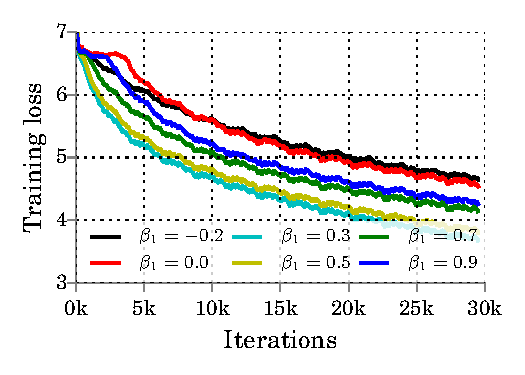
\includegraphics[width=0.45\linewidth]{experiment_results/ptb/adam_stale_15_tuning.pdf} &
%%		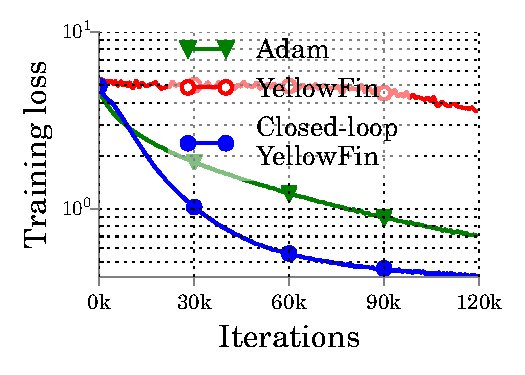
\includegraphics[width=0.45\linewidth]{experiment_results/resnet/resnet_bottleneck_cmp_tuner_adam.pdf}
%%	\end{tabular}
%%	\caption{
%%	Hand-tuning Adam's momentum under asynchrony (left) on PTB LSTM. Asynchronous performance comparison (right) on CIFAR100 ResNet.}
%%	\label{fig:adam_under_staleness}
%%\end{figure}




 







 


